\begin{figure}
	\centering
	\begin{minipage}{.5\textwidth}
	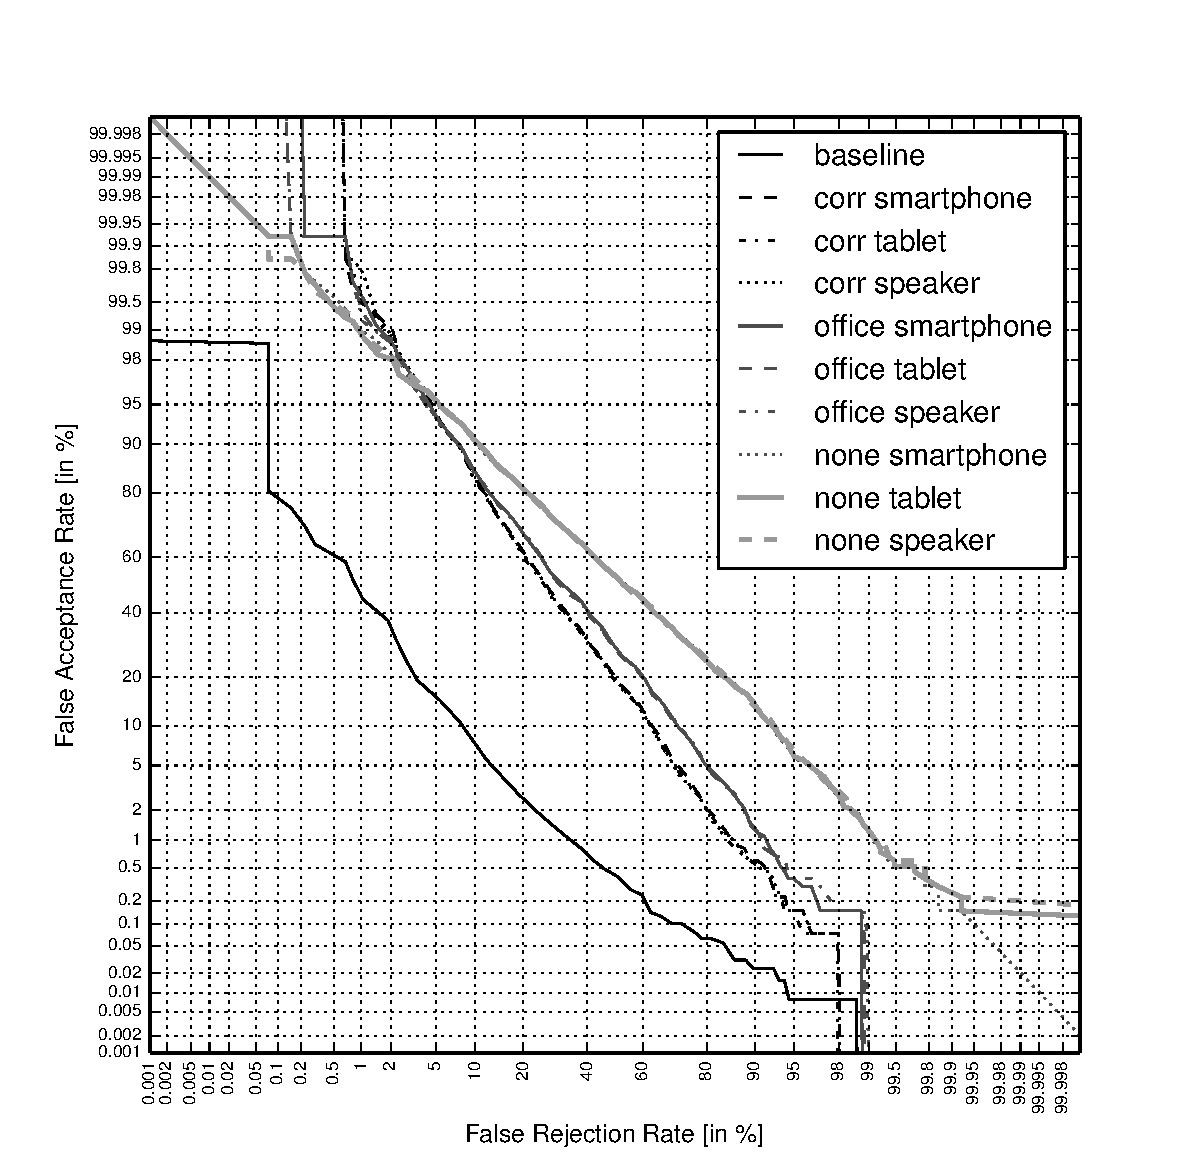
\includegraphics[width=1\linewidth]{Figs/DETs_GMM.pdf}
	\caption{DET plots for the GMM-UBM system for various replay configurations, compared to the baseline performance.}
	\label{fig::DETs_replay_GMM}
	\end{minipage}
	\begin{minipage}{.5\textwidth}
	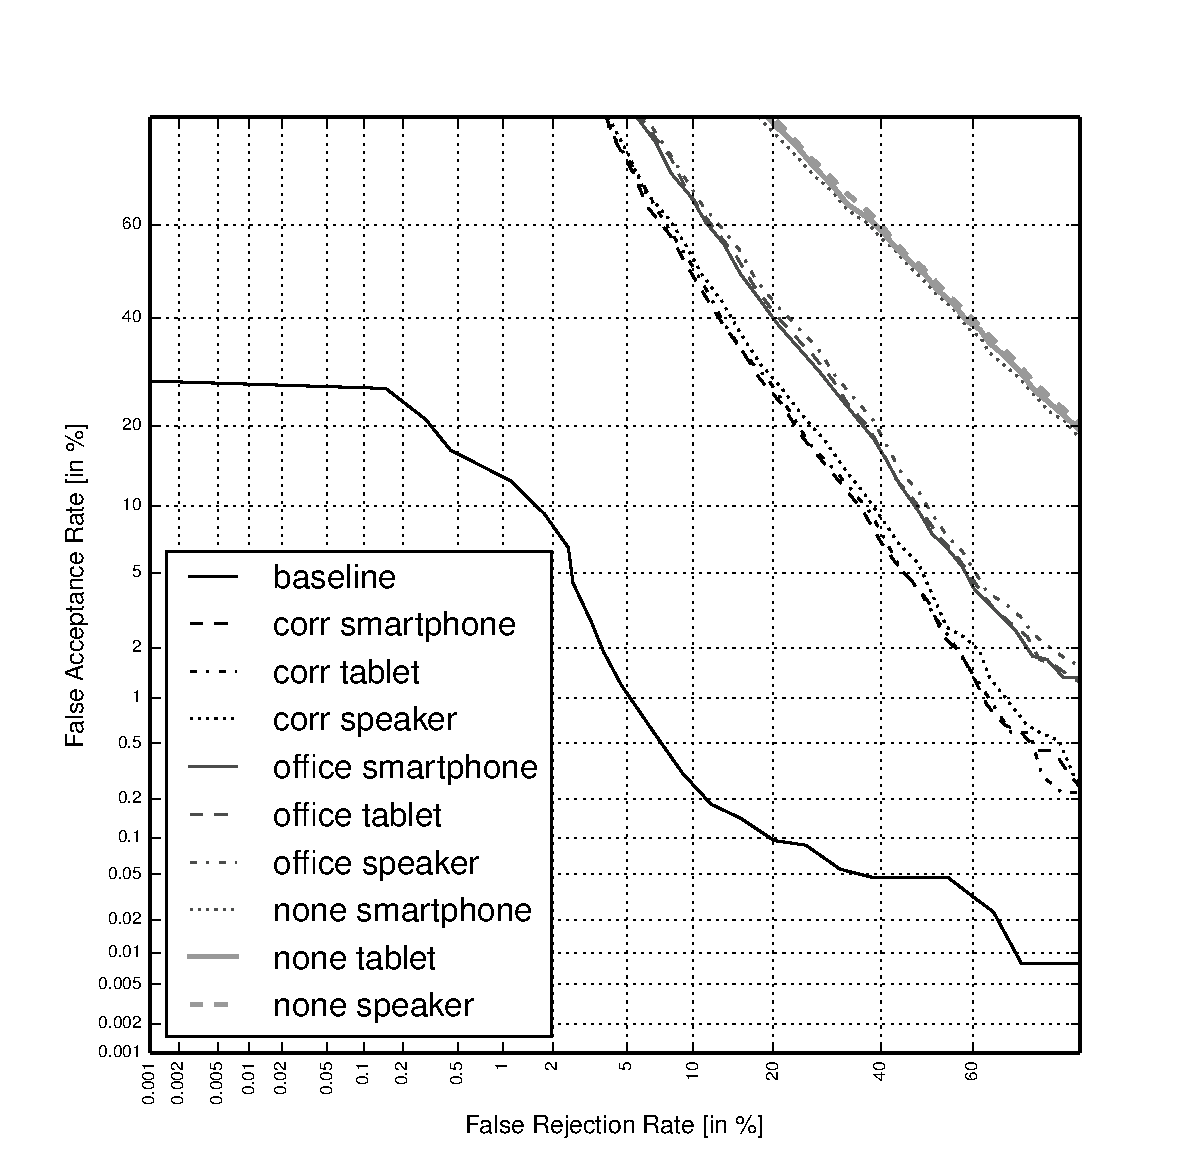
\includegraphics[width=1\linewidth]{Figs/DETs_IV.pdf}
	\caption{DET plots for the IV-PLDA system for various replay configurations, compared to the baseline performance.}
	\label{fig::DETs_replay_IV}
	\end{minipage}


\end{figure}



\begin{figure}
	\centering
	\begin{minipage}{.5\textwidth}
	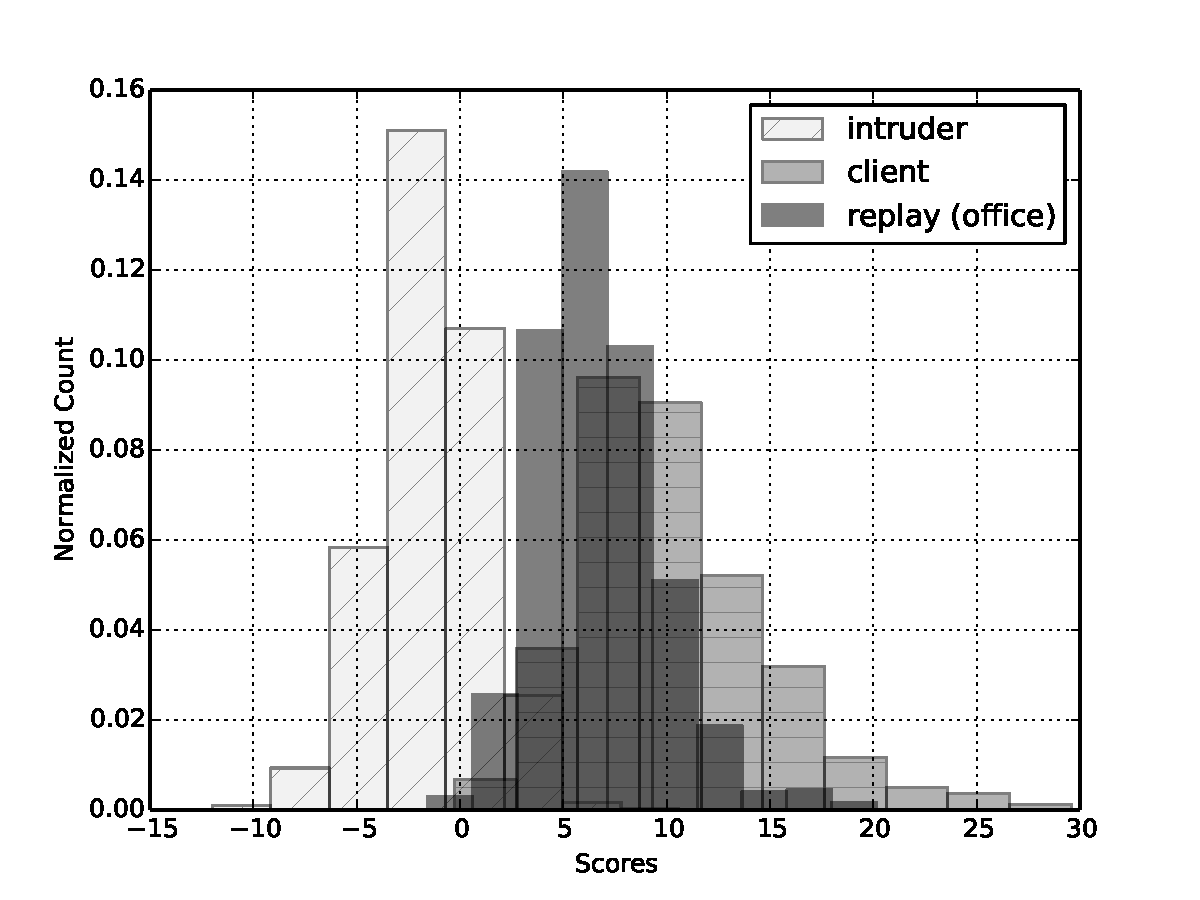
\includegraphics[width=1\linewidth]{Figs/dist_IV_off.pdf}
	\end{minipage}

%	\begin{minipage}{0.5\textwidth}
%	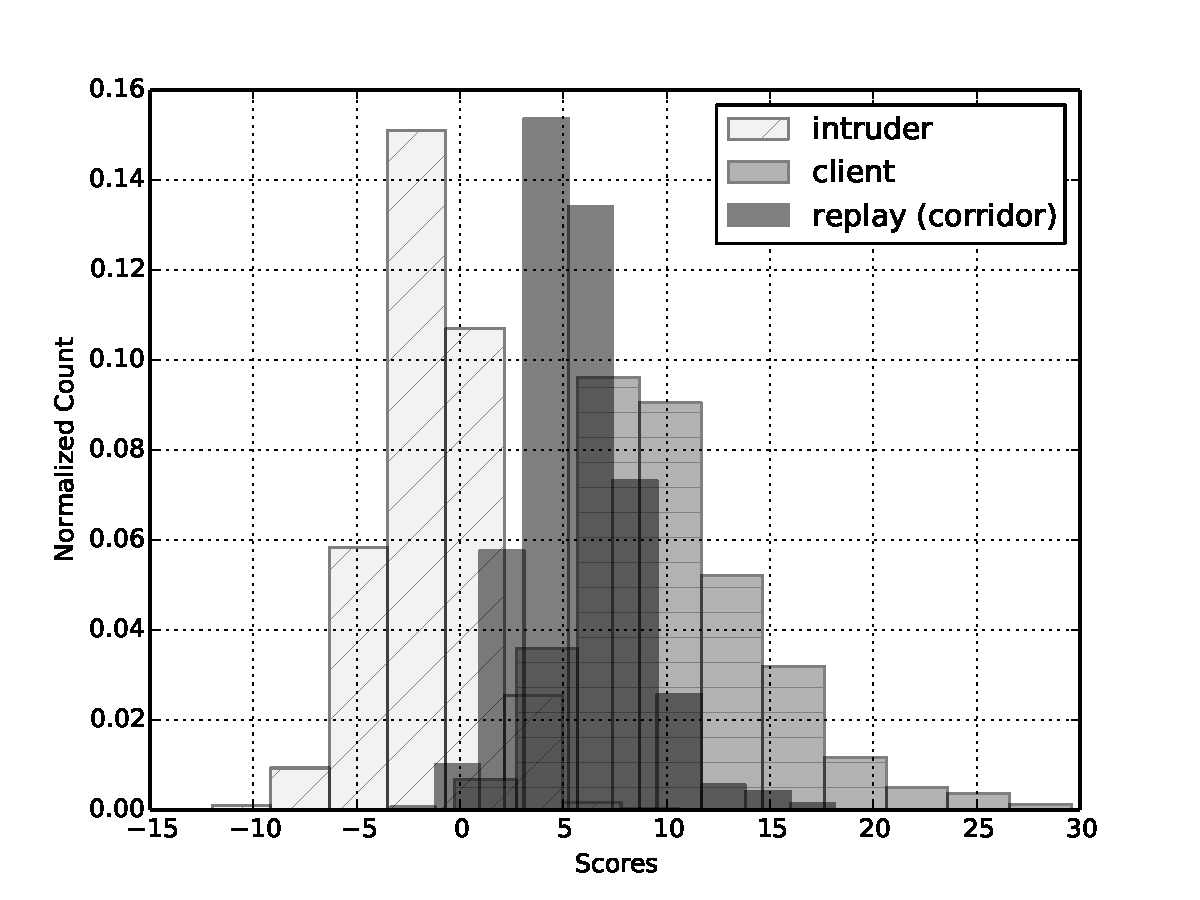
\includegraphics[width=1\linewidth]{Figs/dist_IV_corr.pdf}
%	\end{minipage}
%
%	\begin{minipage}{0.5\textwidth}
%	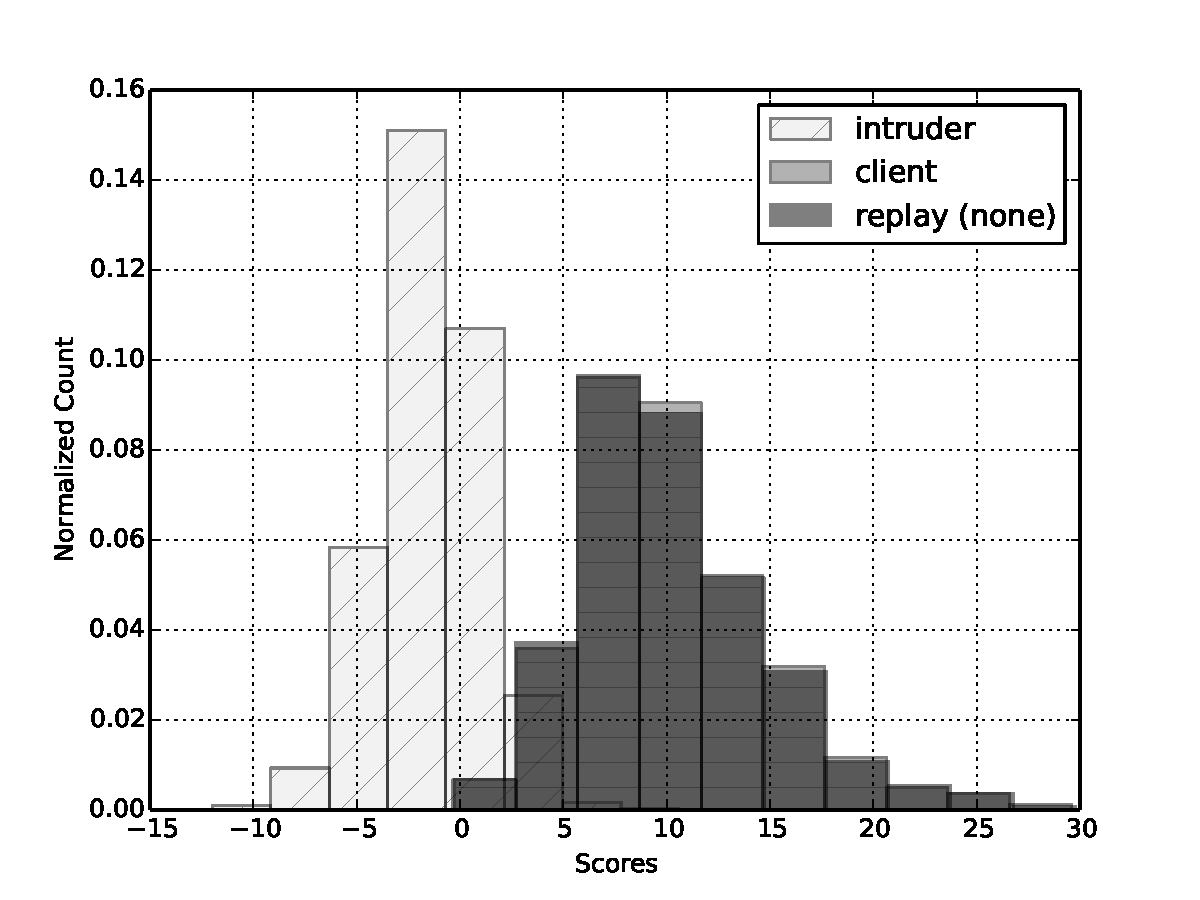
\includegraphics[width=1\linewidth]{Figs/dist_IV_none.pdf}
%	\end{minipage}

	\caption{Score distribution for the IV-PLDA system for replay attacks using a stand-alone speaker and emulation of an office.}
	\label{fig::Dist_IV}
\end{figure}

%\subsubsection{Far-field detection} 

The far-field channel detection countermeasure was implemented according to the algorithm originally proposed in~\cite{Villalba2011} and described in Section~\ref{subsec:ffd}. The total modulation index was calculated from the speech signal envelope which is approximated by the absolute value of the signal after down-sampling to 60~Hz.  The average modulation index was calculated from speech frames whose index is above 0.75.  {\bfseries I struggle to see the correspondence with this description and the one in Section~\ref{subsec:ffd}.  There, there is no mention of average modulation index, where as here there is no mention of spectral ratio, low frequency ratio and the sub-band modulation indices.}




%\subsubsection{LBP setup} 


The LBP countermeasure was implemented using the toolkit provided by The University of Oulu\footnote{http://www.cse.oulu.fi/CMV/Downloads/LBPMatlab}.
Normalised acoustic features used for LBP analysis were composed of 51 coefficients: 16 LFCCs and energy plus their corresponding delta and delta-delta coefficients.  Analysis is based on speech frames and using only the $58$ so-called uniform LBPs\footnote{The subset of LBPs which contain at most two bitwise transitions from 0 to 1 or 1 to 0 when the bit pattern is traversed in circular fashion} as originally described in~\cite{Ojala2002} and for speech processing in~\cite{Alegre2013a}.  {\bfseries wasn't there some prior work by Chatlanni et al?}  LBP histograms are created for all but the first and last frames, thereby obtaining a $58 \times 49 = 2842$ length feature vector for each vector. {\bfseries where does the 49 come from?  To what does a frame refer?  For me, a frame is time-dependent so I don't understand how the 49 is fixed???}

% This is too much detail for something available elsewhere - but we could do with a least some mention of what is a uniform LBP
%Compared to the original implementation, we reduced the number of possible patterns according to the standard Uniform LBP approach. Uniform LBPs are the subset of $58$ patterns which contain at most two bitwise transitions from 0 to 1 or 1 to 0 when the bit pattern is traversed in circularly fashion.  As an example, the subset includes patterns $00000001$ and $00111100$ but not $00110001$.  As reported by~\cite{Ojala2002}, most patterns are naturally uniform and empirical evidence suggests that their use in many image recognition applications leads to better performance then the full set of uniform and non-uniform patterns.  We observed similar findings in our previous work~\cite{Alegre2013a} and thus decided to ignore pixels corresponding to any of the 198 non-uniform patterns.



%\subsubsection{Training the replay detectors} 

Both countermeasure algorithms were trained using a random subset of 1000 utterances from the NIST'05 dataset which were treated as described in Section~\ref{} in order to generate suitable training data with various acoustic conditions.  {\bfseries So there is some overlap here!  Wouldn't it have been better to use different speaker from NIST'04 or NIST'08?} Room and loudspeaker impulse responses (a lecture room, a staircase and a meeting room) different to those used for ASV experiments ensure no countermeasure over-fitting.
%   of replay attack. Therefore we emulated the following environment:
%\begin{itemize}
%\item a lecture room, with concrete walls, glass windows and a parquet;
%\item a staircase, with concrete walls and steps;
%\item a meeting room, with concrete walls, glass windows and a carpet.
%\end{itemize}
%Similarly to emulation of replay attack, the corresponding impulse responses were taken from the AIR database. To train the far-field recording detector, we also needed to emulate the replay device. 
%A single high-quality speaker impulse response was used for We chose a stand-alone speaker impulse response, different from the one used for replay attack emulation, to avoid overfitting to testing data. Original NIST'05 recordings were used to model the licit client access trials.

A binary support vector machines (SVM) classifier with 3rd order polynomial kernel was learned to differentiate genuine data from spoofed data in the case of the far-field channel detection countermeasure.  In contrast, a decision table classifier was used for the LBP countermeasure.  These classifiers returned the best results in each case for an area-under-the-ROC metric.  %Having been trained, both classifiers were applied to detect replay attacks in both spoofing accesses and licit client trials.
